\documentclass[a4paper,12pt]{article}

\usepackage{mystyle}

\usepackage{gensymb}
\usepackage{scalerel}
\usepackage{stackengine}


\graphicspath{ {images/} }


% https://tex.stackexchange.com/questions/5461/is-it-possible-to-change-the-size-of-an-arrowhead-in-tikz-pgf
\usetikzlibrary{arrows.meta}


\DeclareMathOperator{\Image}{Im}

\definecolor{pink}{RGB}{218, 3, 174}
\definecolor{violet}{RGB}{148, 0, 211}
\definecolor{green}{RGB}{0, 153, 0}
\definecolor{orange}{RGB}{255, 153, 0}
\definecolor{blue}{RGB}{5, 73, 255}


% https://tex.stackexchange.com/a/101138/135045

\newcommand\widesim[1]{\ThisStyle{%
  \setbox0=\hbox{$\SavedStyle#1$}%
  \stackengine{-.1\LMpt}{$\SavedStyle#1$}{%
    \stretchto{\scaleto{\SavedStyle\mkern.2mu\sim}{.5150\wd0}}{.6\ht0}%
  }{O}{c}{F}{T}{S}%
}}


\newcommand{\BigMiddleThree}{\;\left|\vphantom{\begin{pmatrix} 0\\0\\0 \end{pmatrix}}\right.\;}
\newcommand{\BigMiddleFour}{\;\left|\vphantom{\begin{pmatrix} 0\\0\\0\\0 \end{pmatrix}}\right.\;}


% https://tex.stackexchange.com/questions/63531/how-to-write-quotation-marks-in-math-environment
\DeclareMathSymbol{\mlq}{\mathord}{operators}{``}
\DeclareMathSymbol{\mrq}{\mathord}{operators}{`'}


\DeclareMathOperator{\Imag}{Im}


% https://tex.stackexchange.com/questions/544453/undefined-control-sequence-after-paragraph
\renewcommand{\paragraph}[1]{\noindent\textbf{#1}\quad}


% https://tex.stackexchange.com/questions/36851/skipping-line-after-proof-in-proof-environment#comment73553_36851
\newcommand{\proofindent}{\hspace*{\fill}\par\vspace{0.5em}\noindent}


% https://tex.stackexchange.com/questions/4813/extendible-equals-sign
\makeatletter
\newcommand*{\Relbarfill@}{\arrowfill@\Relbar\Relbar\Relbar}
\newcommand*{\xeq}[2][]{\ext@arrow 0055\Relbarfill@{#1}{#2}}
\makeatother


% https://tex.stackexchange.com/questions/279100/typeset-the-shrug-%C2%AF-%E3%83%84-%C2%AF-emoji
\newcommand{\shrug}[1][]{%
\begin{tikzpicture}[baseline,x=0.8\ht\strutbox,y=0.8\ht\strutbox,line width=0.125ex,#1]
  \def\arm{(-2.5,0.95) to (-2,0.95) (-1.9,1) to (-1.5,0) (-1.35,0) to (-0.8,0)};
  \draw \arm;
  \draw[xscale=-1] \arm;
  \def\headpart{(0.6,0) arc[start angle=-40, end angle=40,x radius=0.6,y radius=0.8]};
  \draw \headpart;
  \draw[xscale=-1] \headpart;
  \def\eye{(-0.075,0.15) .. controls (0.02,0) .. (0.075,-0.15)};
  \draw[shift={(-0.3,0.8)}] \eye;
  \draw[shift={(0,0.85)}] \eye;
  % draw mouth
  \draw (-0.1,0.2) to [out=15,in=-100] (0.4,0.95); 
\end{tikzpicture}}


% Source: https://svgsilh.com/image/3414775.html (the small one)
% TODO: white rectangles hiding original rope
\newcommand{\baloon}{\resizebox{\fontcharht\font`M}{!}{
\includegraphics{baloon}}}


\theoremstyle{remark}
\newtheorem*{finalsolution}{Решение}
\AtEndEnvironment{finalsolution}{\newline\null\hfill\baloon}  % TODO: float image on the same line without a new one (quite big picture -> last line seems like it's after vertical indent)



\author{Алексеев Василий}


\title{Семинар 12}
\date{28 апреля + 2 мая 2023}


\begin{document}
  \maketitle
  
  \tableofcontents

  \thispagestyle{empty}
  
  \newpage
  
  
  
  \vspace*{\fill}
  
  \noindent
  \emph{Некоторые ``договорённости'' (предварительные уточнения):}
  
  \begin{itemize}
    \item \emph{
      Жирным шрифтом обозначаются как векторы линейного пространства, так и их координатные столбцы в выбранном базисе.
      При этом и векторы, и их координатные столбцы обозначаются, как правило, одинаковыми буквами.
      Например, $\bds x \hm\in X$ (вектор) и $\bds x \hm\in \RR^{\dim X}$ (его координатный столбец).
      Таким образом, смысл зависит от контекста
    } \shrug
  
    \item \emph{
      Билинейная функция называется именно ``билинейной функцией''.
      Хотя общепринятым синонимом является также термин ``билинейная форма''.
      Квадратичная же функция иногда в конспекте именуется и ``квадратичной формой'' (общепринятый синоним), и даже просто ``формой'' (немного неряшливое короткое обозначение, которое, однако, можно считать корректным, но только в рамках конспекта~---~неопределённости возникнуть не должно, потому что билинейная функция ``формой'' именоваться не будет).
    }
  \end{itemize}
  
  \vspace*{\fill}
  
  \thispagestyle{empty}
  
  \newpage
  
  
  \pagenumbering{arabic}


  \section{Inn + Li = Bili (Diag E2)}
  
  
  \subsection{Карта диагонализаций}
  
  Вспомним кратко рассмотренные ранее ``сюжеты о диагонализации''~(\ref{fig:diag-scheme}).
  Распишем тезисно о каждом основные моменты: ``где'', ``что'', ``когда'' и ``как''.
  
  \begin{figure}[h]
    \centering
    
    % TODO: sorry but this picture looks a bit "cheap"
    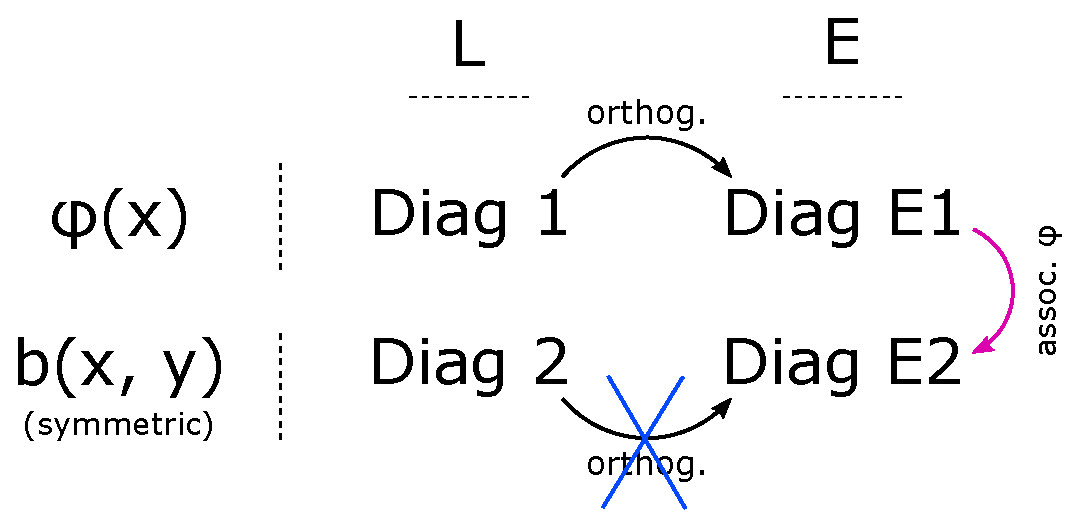
\includegraphics[width=0.7\columnwidth]{diag-scheme}
    
    \caption{``Карта диагонализаций'' в виде таблицы. По строкам~---~``что'' (линейное преобразование или симметричная билинейная функция), по столбцам~---~``где'' (``просто'' линейное пространство или евклидово). В ячейках~---~заголовки соответствующих конспектов. \emph{Diag~1}, \emph{Diag~2}, \emph{Diag~E1}~---~пройденные, \emph{Diag E2}~---~текущий. Подписи стрелок: \emph{orthog.} означает ``orthogonalization'' (ортогонализация системы векторов по Граму~--~Шмидту), \emph{assoc.~$\phi$} означает ``associated~$\phi$'' (присоединённое преобразование~---~подробнее о нём будет далее в конспекте).}
    \label{fig:diag-scheme}
  \end{figure}
  
  \emph{Diag 1}.
  Линейное пространство~$\mathcal L$, в нём выбран базис~$e \hm= (\bds e_1, \ldots, \bds e_n)$.
  Линейное преобразование~$\phi(\cdot)$ с матрицей~$A$ в базисе~$e$.
  \emph{Если} найдётся базис~$e' \hm= e S$ из собственных векторов преобразования~$\phi(\cdot)$, то матрица~$A'$ преобразования в этом базисе будет диагональной (с собственными значениями~$\lambda_i$ на диагонали):
  \begin{equation}\label{eq:diag1-matrix-change}
    A' = S^{-1} A S = \diag(\lambda_1, \ldots, \lambda_n)
  \end{equation}
  
  Базис из собственных векторов обязательно найдётся, если у преобразования~$\phi$ есть~$n$ \emph{различных} собственных значений.
  (Это достаточное условие, но не необходимое.)
  
  \smallskip
  
  \emph{Diag 2}.
  Линейное пространство~$\mathcal L$, в нём выбран базис~$e$.
  Билинейная симметричная функция~$b(\cdot, \cdot)$ с матрицей~$B$ в базисе~$e$.
  \emph{Всегда} найдётся базис~$e' \hm= e S$, в котором матрица~$B'$ билинейной функции будет диагональной, более того~---~будет иметь канонический вид (когда на диагонали стоят только числа $\eps_i \hm\in \{\pm 1, 0\}$):
  \begin{equation}\label{eq:diag2-matrix-change}
    B' = S^T B S = \diag(\eps_1, \ldots, \eps_n)
  \end{equation}
  
  Для нахождения базиса~$e'$ можно либо проводить попеременные одинаковые элементарные преобразования столбцов и строк матрицы билинейной функции, либо использовать \emph{метод Лагранжа} выделения квадратов в формуле квадратичной функции и последующих замен переменных.
  
  \smallskip
  
  \emph{Diag E1}.
  Евклидово пространство~$\mathcal E$, в нём выбран базис~$e$.
  \emph{Самосопряжённое} преобразование~$\phi(\cdot)$ с матрицей~$A$ в базисе~$e$.
  \emph{Всегда} найдётся \emph{ортонормированный} базис~$e' \hm= e S$ из собственных векторов преобразования~$\phi(\cdot)$ (и матрица~$A'$ преобразования в этом базисе будет диагональной с собственными значениями~$\lambda_i$ на диагонали, и при смене базиса меняется как~(\ref{eq:diag1-matrix-change})).
  Для того чтобы получить этот ортонормированный базис, достаточно просто провести \emph{ортогонализацию} и нормировку базиса из собственных векторов.
  
  \smallskip
  
  И тема текущего конспекта (``последний ``сюжет о диагонализациях'').
  
  \smallskip
  
  \emph{Diag E2}.
  Евклидово пространство~$\mathcal E$, в нём выбран базис~$e$.
  Билинейная симметричная функция~$b(\cdot, \cdot)$ с матрицей~$B$ в базисе~$e$.
  Найдётся ли \emph{ортонормированный} базис~$e' \hm= e S$, в котором матрица~$B'$ билинейной функции будет диагональной?
  
  Ответ~---~да, найдётся, причём \emph{всегда}.
  Однако способ поиска этого ортонормированного базиса, как ни странно это могло бы показаться, никак не будет связан с базисом в линейном пространстве, где матрица квадратичной формы имела канонический вид~(\ref{eq:diag2-matrix-change}).
  
  \begin{example}[Иллюстрация того, что ортогонализация в случае квадратичных форм ``не помогает'']
    Пусть $b(\cdot, \cdot)$ есть симметричная билинейная функция на двумерном евклидовом пространстве.
    Пусть удалось найти базис~$e \hm= (\bds e_1, \bds e_2)$, в котором~$b(\cdot, \cdot)$ имеет канонический вид, и пусть её матрица~$B$ при этом есть:
    \[
      B = \begin{pmatrix}
        1 & 0\\
        0 & 1
      \end{pmatrix}
    \]
    
    Допустим, что для того, чтобы из базиса~$e$ получить ортогональный~$e'$, надо выполнить следующее преобразование:
    \[
      e' = (\bds e_1, \bds e_2 - \bds e_1) = e S,\ S = \begin{pmatrix}
        1 & -1\\
        0 & 1
      \end{pmatrix}
    \]
    (Вычитание из одного вектора его ортогональной проекции на другой~---~совершенно ``обычное'' преобразование при ортогонализации системы векторов по Граму~--~Шмидту.)
    
    Как при этом изменится матрица~$B'$ билинейной функции?
    \[
      B' = S^T B S = \begin{pmatrix}
        1 & 0\\
        -1 & 1
      \end{pmatrix}
      \begin{pmatrix}
        1 & 0\\
        0 & 1
      \end{pmatrix}
      \begin{pmatrix}
        1 & -1\\
        0 & 1
      \end{pmatrix} = \begin{pmatrix}
        1 & -1\\
        -1 & 2
      \end{pmatrix}
    \]
    
    Диагональность ``потеряна''.
    (И при нормировке векторов~$e'$ она тоже не вернётся.)
    Таким образом, то, что получилось с преобразованиями (найти ОНБ путём ортогонализации базиса), с квадратичными формами ``не проходит''...
  \end{example}
  
  Оказывается, что для того, чтобы найти ОНБ для диагонального вида симметричной билинейной функции, надо снова искать собственные значения и собственные векторы...
  Собственные векторы~---~но какого линейного преобразования?
  
  
  \subsection{Присоединённое преобразование}
  
  \begin{definition}
    Пусть есть евклидово пространство~$\mathcal E$ и симметричная билинейная функция~$b(\cdot, \cdot)\colon \mathcal E \hm\times \mathcal E \hm\to \RR$.
    Тогда \emph{присоединённым к $b(\cdot, \cdot)$ преобразованием}\footnote{
      Автору конспекта не удалось найти аналог этого термина в англоязычных ресурсах...
      Встречалось название ``associated'' (см. \href{https://community.ams.org/journals/tran/1968-131-02/S0002-9947-1968-0221299-7/S0002-9947-1968-0221299-7.pdf}{McIntosh, A. (1968). \emph{Representation of bilinear forms in Hilbert space by linear operators}. Transactions of the American Mathematical Society}).
      Но есть сомнения, что это ``общепринятый'' термин.
      (На самом деле те же сомнения есть и относительно самого термина ``присоединённое преобразование''.)
      Anyway...
      А вообще, не только к \emph{симметричной} билинейной функции можно ``присоединить'' преобразование.
      Если есть произвольная билинейная функция~$b(\cdot, \cdot)$, то можно и её представить в виде~$b(\bds x, \bds y) \hm= (\bds x, \phi(\bds y))$, где~$\phi(\cdot)$ есть линейное преобразование (если $b(\cdot, \cdot)$ симметричная, то~$\phi$ как раз называется присоединённым).
      Подробнее см. \href{https://linalge.page.link/Ershov_LA_2022}{лекции Ершова~А.~В., глава 10.4. \emph{Связь между линейными операторами и билинейными функциями на евклидовом пространстве}}.
      Более того, билинейной функции можно сопоставить линейное \emph{отображение} (не преобразование) и просто в линейном пространстве, не только в евклидовом!
      Так, пусть~$\bds x_0$~---~некоторый фиксированный вектор линейного пространства~$\mathcal L$.
      Тогда, имея билинейную функцию~$b(\cdot, \cdot)$ на этом пространстве~$\mathcal L$, можно определить следующие линейные отображения: ``левое'' $f_{l}\colon \mathcal L \hm\ni \bds x \hm\mapsto b(\bds x_0, \bds x) \hm\in \RR$ и ``правое'' $f_{r}\colon \mathcal L \hm\ni \bds x \hm\mapsto b(\bds x, \bds x_0) \hm\in \RR$.  % Better would be `f_{\bds x_0, l}` but it is hard to read (especially as a footnote)
      Что получается: выбираем один вектор~$\bds x_0$, и можем с помощью билинейной функции получить два линейных отображения (``левое'' и ``правое''), выбираем другой вектор~$\bds x_0'$~---~и получаем другие линейные отображения.
      То есть имеем два соответствия между векторами~$\mathcal L$ и линейными функциями на~$\mathcal L$ (составляющими \emph{сопряжённое} пространство~$\mathcal L^*$): ``левое'' $\phi_l\colon \mathcal L \hm\ni \bds x \hm\mapsto f_{l} \hm\in \mathcal L^*$ и ``правое'' $\phi_r\colon \mathcal L \hm\ni \bds x \hm\mapsto f_{r} \hm\in \mathcal L^*$.
      Итого, каждой билинейной функции~$b(\cdot, \cdot)$ можно поставить в соответствие отображения $\phi_l$ и $\phi_r$.
      Подробнее см. \href{https://kconrad.math.uconn.edu/blurbs/linmultialg/bilinearform.pdf}{\emph{листочек Кейта Конрада (Keith Conrad) по билинейным формам} (конец первого раздела и начало второго)}.
    } называется линейное преобразование~$\phi\colon \mathcal E \hm\to \mathcal E$, такое что:
    \begin{equation}\label{eq:assoc-phi}
      b(\bds x, \bds y) = (\bds x, \phi(\bds y)),\quad \forall \bds x, \bds y \in \mathcal E
    \end{equation}
  \end{definition}
  
  Так как билинейная функция $b(\cdot, \cdot)$ предполагается симметричной, и так как скалярное произведение симметрично, можно из~(\ref{eq:assoc-phi}) можно получить:
  \[
    (\bds x, \phi(\bds y)) = b(\bds x, \bds y) = b(\bds y, \bds x) = (\bds y, \phi(\bds x)) = (\phi(\bds x), \bds y)
    \Rightarrow \underline{(\phi(\bds x), \bds y) = (\bds x, \phi(\bds y))}
  \]

  \begin{proposition}\label{theo:assoc-is-self-adjo}
    Преобразование, присоединённое к симметричной билинейной функции, является самосопряжённым.
  \end{proposition}

  Но найдётся ли вообще для данной симметричной билинейной функции~$b(\cdot, \cdot)$ присоединённое преобразование?\footnote{Иначе ``не очень хорошо'' получается: обсуждать свойства того, чего нет.}
  Если оно есть, то обязательно ли единственное? или может быть несколько присоединённых?

  Пусть $e \hm= (\bds e_1, \ldots, \bds e_n)$ это базис в $\mathcal E$.
  Пусть матрица~$\Gamma$ это матрица Грама базиса~$e$, матрица $B$ это матрица билинейной функции $b(\cdot, \cdot)$, а матрица~$A$~---~матрица присоединённого к $b(\cdot, \cdot)$ преобразования~$\phi(\cdot)$ (предполагаем, что оно существует, и тогда~$A$ есть его матрица).

  Перепишем~(\ref{eq:assoc-phi}) в терминах матриц и вектор-столбцов:
  \[
    \bds x^T B \bds y = \bds x^T \Gamma (A \bds y)
    \leftrightarrow \bds x^T B \bds y = \bds x^T (\Gamma A) \bds y
  \]

  Соотношение выше верно для любой пары векторов $\bds x$, $\bds y$.
  Это значит, что должны быть равны матрицы ``посередине'':
  \begin{equation}\label{eq:assoc-phi-matrix}
    B = \Gamma A \Rightarrow \boxed{A = \Gamma^{-1} B}
  \end{equation}
  (где было использовано, что матрица Грама базиса невырождена, поэтому обязательно существует её обратная~$\Gamma^{-1}$).
  
  \begin{proposition}
    Для любой симметричной билинейной функции в евклидовом пространстве существует и единственно присоединённое к ней преобразование.
  \end{proposition}
  
  Если базис в~$\mathcal E$ выбран ортонормированным, то связь между матрицами билинейной функции и присоединённого к ней преобразовния~(\ref{eq:assoc-phi-matrix}) станет:
  \begin{equation}
    \boxed{A = B\quad \mbox{(ОНБ)}}
  \end{equation}
  то есть \emph{в ортонормированном базисе матрицы билинейной функции и присоединённого к ней пребразования совпадают}.
  
  Хорошо, присоединённое преобразование самосопряжённое, и потому у него есть ортонормированный базис из собственных векторов, где его матрица диагональная...
  Но как это помогает в поиске ортонормированного базиса, в котором диагональна \emph{квадратичная форма}?

  
  % TODO: need new page because title appears at the end of page
  
  \newpage
  
  \subsection{Последняя глава о диагонализациях}
  
  \noindent
  \textbf{Исходный ОНБ (``хороший случай'')}

  Пусть в $\mathcal E$ выбран \emph{ортонормированный} базис $e \hm= (\bds e_1, \ldots, \bds e_n)$.
  (То есть матрица Грама базиса $\Gamma \hm= E$.)
  Пусть $b(\cdot, \cdot)$ есть симметричная билинейная функция, а $\phi(\cdot)$~---~это присоединённое к ней преобразование.
  (Тогда матрица~$A$ преобразования совпадает с матрицей~$B$ билинейной функции.)

  Так как присоединённое преобразование~$\phi$ самосопряжённое~(\ref{theo:assoc-is-self-adjo}), то для него \emph{обязательно найдётся ортонормированный базис из собственных векторов}.
  Пусть $e'$ есть этот базис, и~$S$~---~матрица перехода от исходного \emph{ортонормированного базиса~$e$} к этому новому (\emph{тоже ортонормированному}) базису~$e'$:
  \begin{equation}\label{eq:from-orthogo-to-orthogo-basis}
    e' = e S
  \end{equation}
  
  Что значит, что базис~$e'$ ортонормированный?
  Это значит, что, например:
  \begin{equation}\label{eq:orthogo-vectors-in-basis}
    \left\{
      \begin{aligned}
        &(\bds e_1', \bds e_1') = \bds e_1^{\prime T} \bds e_1' = 1\\
        &(\bds e_1', \bds e_2') = \bds e_1^{\prime T} \bds e_2' = 0\\
        &\ldots\\
        &(\bds e_1', \bds e_n') = \bds e_1^{\prime T} \bds e_n' = 0\\
      \end{aligned}
    \right.
  \end{equation}
  
  То есть \emph{если записать координаты вектора $\bds e_1'$ в базисе $e$ в строчку, и умножить эту строчку на матрицу из координатных столбцов векторов $e'$ в базисе $e$, то получится первый столбец единичной матрицы}.
  % TODO: picture
  Аналогично можно рассмотреть скалярные произведения вектора $\bds e_2'$ на все векторы базиса $e'$ и так далее.
  Приходим к соотношению:
  \begin{equation}\label{eq:matrix-fr}
    S^T S = E \Rightarrow \underline{S^{-1} = S^T}
  \end{equation}
  то есть \emph{матрица перехода от одного ортонормированного базиса к другому ортонормированному базису ортогональна}.
  
  Раз $e'$ это ортонормированный базис из собственных векторов присоединённого преобразования~$\phi$, то матрица~$A'$ преобразования~$\phi$ в этом базисе будет равна:
  \[
    A' = S^{-1} A S = D
  \]
  где~$D$ означает диагональную матрицу, на диагонали которой стоят собственные значения преобразования~$\phi$, соответствующие векторам базиса~$e'$.
  
  С другой стороны, матрица~$B'$ билинейной функции $b$ при смене базиса:
  % TODO: picture scheme
  \begin{equation}\label{eq:diag-bili-in-new-basis}
    B' = S^T B S \xeq[B = A]{S^{-1} = S^T} S^{-1} A S = D
  \end{equation}
  то есть матрица~$B'$ тоже диагональная!
  и такая же, как матрица $A'$, то есть на её диагонали стоят собственные значения присоединённого преобразования~$\phi$.


  \bigskip
  \noindent
  \textbf{Исходный не ОНБ (``общий случай'')}
  
  Пусть в $\mathcal E$ выбран \emph{некоторый} базис $e \hm= (\bds e_1, \ldots, \bds e_n)$.
  (То есть матрица Грама базиса $\Gamma$ не обязательно единичная.)
  Пусть $b(\cdot, \cdot)$ есть симметричная билинейная функция.
  (С симметричной матрицей~$B$ в базисе~$e$.)
  
  Можно ли в этом случае найти ортонормированный базис, где бы матрица билинейной функции была диагональна?
  Да, можно.
  
  \medskip
  
  \emph{Способ 1: сначала к ОНБ, потом ``по-простому''}.
  
  Раз в случае ОНБ базиса всё понятно, то можно просто сначала перейти к какому-нибудь ОНБ.
  Пусть $e'$~---~это некоторый ортонормированный базис:
  \[
    e' = e S_1
  \]
  
  При переходе от исходного (не факт, что ортонормированного) базиса~$e$ к новому~$e'$ матрица билинейной функции~$b$ изменяется:
  \[
    B' = S_1^T B S_1
  \]
  
  Теперь, находясь в ортонормированном базисе~$e'$, можем сделать всё так же, как раньше~(\ref{eq:diag-bili-in-new-basis}): перейти к ортонормированному базису~$e''$ из собственных векторов присоединённого к билинейной функции~$b$ преобразования~$\phi$ (с матрицей $A' \hm= B'$ в базисе~$e'$):
  \[
    e'' = e' S_2,\ S_2^{-1} = S_2^T,\quad A'' = B'' = D
  \]
  
  Итого, матрица перехода~$S$ от исходного базиса~$e$ к ортонормированному~$e''$, где матрица билинейной функции диагональная:
  \[
    e'' = e' S_2 = e S_1 S_2 \Rightarrow \underline{S = S_1 S_2}
  \]
  
  \medskip
  
  \emph{Способ 2: сразу ``как надо''}.
  
  Пусть~$\phi$~---~это присоединённое к билинейной функции~$b$ преобразование.
  (Тогда матрица преобразования есть $\underline{A \hm= \Gamma^{-1} B}$.)
  
  Присоединённое к билинейной~---~обязательно самосопряжённое~(\ref{theo:assoc-is-self-adjo})\footnote{Можно в этом убедиться и в общем базисе: $\bigl(\phi(\bds x), \bds y\bigr) \hm= (A \bds x)^T \Gamma \bds y \hm= \bds x^T A^T \Gamma \bds y \hm= \bds x^T (\Gamma^{-1} B)^T \Gamma \bds y \hm= \bds x^T B^T (\Gamma^{-1})^T \Gamma \bds y \hm= \bds x^T B^T (\Gamma^{-1} \Gamma) \bds y \hm= \bds x^T B^T \bds y \hm= \bds x^T B \bds y \hm= \bds x^T (\Gamma A) \bds y \hm= \bds x^T \Gamma (A \bds y) \hm= \bigl(\bds x, \phi(\bds y)\bigr)$.}.
  Поэтому найдётся ортонормированный базис~$e'$ из собственных векторов~$\phi$:
  \[
    e' = e S
  \]
  В чём ``подвох'', в чём разница по сравнению с~(\ref{eq:from-orthogo-to-orthogo-basis})?
  Разница в том, что базис~$e'$ ортонормированный, но \emph{относительно скалярного произведения с матрицей Грама~$\Gamma$}!
  То есть, если выписывать скалярные между базисными~$e'$ по аналогии с~(\ref{eq:orthogo-vectors-in-basis}):
  \[
    \left\{
      \begin{aligned}
        &(\bds e_1', \bds e_1') = \bds e_1^{\prime T} \Gamma \bds e_1' = 1\\
        &(\bds e_1', \bds e_2') = \bds e_1^{\prime T} \Gamma \bds e_2' = 0\\
        &\ldots\\
        &(\bds e_1', \bds e_n') = \bds e_1^{\prime T} \Gamma \bds e_n' = 0\\
      \end{aligned}
    \right.
  \]
  то станет понятно, что матрица перехода~$S$ должна обладать следующим свойством:
  \[
    \underline{S^T \Gamma S = E}
  \]
  
  В базисе из собственных векторов для матрицы преобразования~$A'$ имеем:
  \[
    A' = S^{-1} A S = D
  \]
  
  Что будет с матрицей билинейной функции~$B'$?
  Она тоже будет диагональной!
  Это видно из ``связки'' между матрицами билинейной функции и присоединённого преобразования ($\Gamma_{e}$ есть та же $\Gamma$ в обозначениях выше):
  \[
    B = \Gamma_{e} A \xrightarrow{e' = e S} B' = \Gamma_{e'} A' = A' = D
  \]
  так как базис~$e'$ ортонормированный, то есть его матрица Грама~$\Gamma_{e'}$ единичная.
  
  Но можно и ``строго'' показать диагональность~$B'$:
  \[
    B' = S^T B S
    = S^T (\Gamma A) S
    = S^T \Gamma (S S^{-1}) A S
    = (\underbrace{S^T \Gamma S}_{\Gamma_{e'}}) (S^{-1} A S)
    = E A'
    = D
  \]
    

  \subsection{Одна форма в евклидовом, или \# 32.27(13)}\label{seq:p32-27}
  
  Квадратичная функция~$k(\cdot)$ задана в \emph{ортонормированном} базисе~$e$ трёхмерного евклидова пространства~$\mathcal E$:
  \[
    k(\bds x) = x_1^2 - x_1 x_2 + x_1 x_3 + x_2^2 + x_2 x_3 + x_3^2
  \]
  
  Надо найти ортонормированный базис, в котором $k(\cdot)$ имеет диагональный вид (и сам этот диагональный вид).
  
  \begin{solution}
    (Раз надо найти \emph{ортонормированный} базис, где форма диагональна, то использовать надо не метод Лагранжа выделения квадратов, а собственные векторы присоединённого преобразования.)
    
    Матрица соответствующей билинейной~$b(\cdot, \cdot)$ функции:
    \[
      B = \begin{pmatrix}
        1    & -1/2 & 1/2\\
        -1/2 & 1    & 1/2\\
        1/2  & 1/2  & 1
      \end{pmatrix}
    \]
    
    Так как базис~$e$ ортонормированный, то у присоединённого к $b(\cdot, \cdot)$ преобразования~$\phi(\cdot)$ будет такая же матрица:
    \[
      A = B
    \]
    
    Найдём собственные значения~$\phi$.
    (Можно заметить, что разность третьей и второй строчки~$A$ даёт первую, поэтому $\lambda \hm= 0$ точно будет собственным значением.)
    \[
      \det(A - \lambda E) = 0 \Rightarrow \ldots \Rightarrow \left[
        \begin{aligned}
          &\lambda = 0\\
          &\lambda = 3/2, \quad \mbox{(кр-ть 2)}
        \end{aligned}
      \right.
    \]
    
    Найдём собственные векторы~$\phi$.
    (Так как $\lambda \hm= 3/2$ это корень кратности~$2$, а у преобразования~$\phi$, как у самосопряжённого, должен найтись базис из собственных векторов, то ожидается, что для $\lambda \hm= 3/2$ получится найти \emph{два} линейно независимых собственных вектора, то есть размерность соответствующего собственного подпространства обязательно также будет равна~$2$.)
    
    При~$\lambda_1 \hm= 0$:
    \[
      (A - \lambda_1 E) \bds x = \bds 0
      \leftrightarrow \begin{pmatrix}
        1    & -1/2 & 1/2\\
        -1/2 & 1    & 1/2\\
        1/2  & 1/2  & 1
      \end{pmatrix} \begin{pmatrix}
        x_1\\
        x_2\\
        x_3
      \end{pmatrix} = \begin{pmatrix}
        0\\
        0\\
        0
      \end{pmatrix}
      \Rightarrow \ldots \Rightarrow \bds x_1 = \begin{pmatrix}
        -1\\
        -1\\
        1
      \end{pmatrix}
    \]
    
    При~$\lambda_2 \hm= 3/2$:
    \[
      (A - \lambda_2 E) \bds x = \bds 0
      \leftrightarrow \begin{pmatrix}
        -1/2 & -1/2 & 1/2\\
        -1/2 & -1/2 & 1/2\\
        1/2  & 1/2  & -1/2
      \end{pmatrix} \begin{pmatrix}
        x_1\\
        x_2\\
        x_3
      \end{pmatrix} = \begin{pmatrix}
        0\\
        0\\
        0
      \end{pmatrix}
      \Rightarrow \ldots \Rightarrow \bds x_2 = \begin{pmatrix}
        -1\\
        1\\
        0
      \end{pmatrix},
      \bds x_3 = \begin{pmatrix}
        1\\
        0\\
        1
      \end{pmatrix}
    \]
    
    Имеем базис из собственных векторов:
    \[
      \{\bds x_1, \bds x_2, \bds x_3\} = \left\{
        \begin{pmatrix}
          -1 \\ -1 \\ 1
        \end{pmatrix},
        \begin{pmatrix}
          -1 \\ 1 \\ 0
        \end{pmatrix},
        \begin{pmatrix}
          1 \\ 0 \\ 1
        \end{pmatrix}
      \right\}
    \]
    
    Но нужен ортонормированный базис из собственных векторов.
    Поэтому получим далее сначала ортогональный базис, а потом отнормируем базисные векторы.
    Видно, что $\bds x_1 \hm\perp \bds x_2, \bds x_3$.
    (Этого стоило ожидать, потому что $\bds x_1$ и $\bds x_2$ (а также $\bds x_1$ и $\bds x_3$) это собственные векторы самосопряжённого преобразования, относящиеся к разным собственным значениям.)
    Остаётся ``поправить'' пару $\bds x_2$ и $\bds x_3$, так как пока $(\bds x_2, \bds x_3) \hm= -1 \hm{\not=} 0$.
    Вычтем, например, из вектора~$\bds x_2$ его ортогональную проекцию на вектор~$\bds x_3$:
    \[
      \bds x_2' = \bds x_2 - \frac{(\bds x_2, \bds x_3)}{|\bds x_3|} \cdot \frac{\bds x_3}{|\bds x_3|}
      = \begin{pmatrix}
        -1 \\ 1 \\ 0
      \end{pmatrix} - \frac{-1}{2} \begin{pmatrix}
        1 \\ 0 \\ 1
      \end{pmatrix}
      = \begin{pmatrix}
        -1/2 \\ 1 \\ 1/2
      \end{pmatrix}
    \]
    (Можно убедиться, что вектор~$\bds x_2'$ при этом также собственный, соответствующий $\lambda_2$~---~ведь он получен как линейная комбинация векторов $\bds x_2$ и $\bds x_3$, лежащих в соответствующем собственном подпространстве.)
    
    Ортогональный базис из собственных векторов:
    \[
      \{\bds x_1, \bds x_2', \bds x_3\} = \left\{
        \begin{pmatrix}
          -1 \\ -1 \\ 1
        \end{pmatrix},
        \begin{pmatrix}
          -1/2 \\ 1 \\ 1/2
        \end{pmatrix},
        \begin{pmatrix}
          1 \\ 0 \\ 1
        \end{pmatrix}
      \right\}
    \]
    
    Далее, несложно получить ортонормированный базис из собственных векторов:
    \begin{equation}\label{p:32-27-new-basis}
      e' = \left\{\frac{\bds x_1}{|\bds x_1|}, \frac{\bds x_2'}{|\bds x_2'|}, \frac{\bds x_3}{|\bds x_3|}\right\}
      = \left\{
        \begin{pmatrix}
          -1/\sqrt{3} \\ -1/\sqrt{3} \\ 1/\sqrt{3}
        \end{pmatrix},
        \begin{pmatrix}
          -1/\sqrt{6} \\ 2/\sqrt{6} \\ 1/\sqrt{6}
        \end{pmatrix},
        \begin{pmatrix}
          1/\sqrt{2} \\ 0 \\ 1/\sqrt{2}
        \end{pmatrix}
      \right\}
    \end{equation}
    
    Матрица перехода~$S$ от исходного~$e$ к новому~$e'$~---~это матрица, столбцы которой есть координаты векторов базиса~$e'$ в базисе~$e$ (по сути матрица~$S$ как раз и была выписана выше~(\ref{p:32-27-new-basis}).)
    Видно, что~$S$ ортогональная: $S^T S \hm= E$ (так как базис~$e'$ ортонормированный относительно стандартного скалярного произведения).
    
    Далее, матрица~$A'$ преобразования~$\phi$ в базисе~$e'$~---~очевидно, диагональная, с собственными значениями на диагонали (первый элемент на диагонали~---~собственное значение, соответствующее первому базисному вектору, и так далее):
    \[
      A' = \begin{pmatrix}
        0 & 0   & 0\\
        0 & 3/2 & 0\\
        0 & 0   & 3/2
      \end{pmatrix}
    \]
    
    Но такой же будет и матрица~$B'$ квадратичной формы!
    Потому что:
    \[
      B' = S^T B S = S^{-1} A S = A'
    \]
    (Хотя ``в процессе'' перехода к~$e'$, на ``промежуточных этапах'', матрица билинейной функции могла и отличаться от матрицы присоединённого преобразования.
    Имеется в виду, что, например, в базисе из собственных векторов~$\{\bds x_1, \bds x_2, \bds x_3\}$ матрица~$\phi$ уже была диагональной, однако $b(\bds x_2, \bds x_3) \hm= -3/2 \hm{\not=} 0$, то есть матрица~$b$ диагональной не была.)
  \end{solution}
  
  
  \subsection{Две формы в линейном, или \# 32.36(4)}
  
  В линейном двумерном пространстве~$\mathcal L$ в базисе~$e$ заданы две квадратичные формы $f(\cdot)$ и $g(\cdot)$:
  \[
    f(\bds x) = 2 x_1 x_2 - x_2^2,
    \quad g(\bds x) = 9 x_1^2 - 10 x_1 x_2 + 3 x_2^2
  \]
  
  Надо проверить, что хотя бы одна из форм является знакоопределённой.
  И найти базис, в котором \emph{обе} формы имели бы диагональный вид (и записать формы в этом базисе).
  
  \begin{finalsolution}
    Какая из форма знакоопределённая?
    Очевидно, не~$f(\cdot)$: при $\bds x \hm= (1, 0)^T \hm{\not=} \bds 0$ получаем $f(\bds x) \hm= 0$.
    (Также можно подобрать векторы, на которых форма принимает значения разных знаков, например: $\bds x \hm= (0, 1) \hm\rightarrow f(\bds x) \hm< 0$ и $\bds x \hm= (1, 1) \hm\rightarrow f(\bds x) \hm> 0$.)
    
    Остаётся проверить, что знакопостоянна форма~$g(\cdot)$:
    \begin{equation}\label{p:32-36-g-as-sum-of-squares}
      g(\bds x) = \left[(3 x_1)^2 - 2 \cdot 3 x_1 \cdot \frac{10}{6} x_2 + \left(\frac{5 x_2}{3}\right)^2\right] - \left(\frac{5 x_2}{3}\right)^2 + 3 x_2^2 = \left(3 x_1 - \frac{5 x_2}{3}\right)^2 + \frac{2}{9} x_2^2 \geq 0
    \end{equation}
    и при этом $g(\bds x) \hm= 0 \hm\leftrightarrow \bds x \hm= \bds 0$.
    То есть форма~$g(\cdot)$ положительно определена.
    (Положительную определённость можно бы было проверить и с помощью матрицы формы и критерия Сильвестра.)
    
    Как теперь найти базис, в котором \emph{обе} формы были бы диагональны?
    
    \medskip
    
    \emph{Способ 1: сначала к ОНБ, потом ``по-простому''}.
    
    ``План'': приведём форму~$g(\cdot)$ к каноническому виду, определим скалярное произведение с помощью формы\footnote{Точнее, с помощью симметричной билинейной функции, порождающей квадратичную форму~$g(\cdot)$.}~$g(\cdot)$ (оно будет ``стандартным''), и потом перейдём к ортонормированному базису из собственных векторов присоединённого к форме~$f(\cdot)$ преобразования (в этом базисе $f(\cdot)$ станет диагональной, а $g(\cdot)$ останется диагональной, так как $g(\cdot)$ задаёт скалярное произведение, а новый базис тоже ортонормированный).
    % TODO: picture/table scheme
    % Actually, maybe we do not need it — the text description is enough
    
    Проводим ``очевидную''~(\ref{p:32-36-g-as-sum-of-squares}) замену:
    \[
      \left\{
        \begin{aligned}
          &x_1' = 3 x_1 - \frac{5 x_2}{3}\\
          &x_2' = \frac{\sqrt{2}}{3} x_2
        \end{aligned}
      \right.
    \]
    
    В новых переменных форма~$g(\cdot)$ имеет канонический вид:
    \[
      g(\bds x) = x_1^{\prime 2} + x_2^{\prime 2}
    \]
    
    Обратная замена (нужна, чтобы получить матрицу перехода~$S_1$ от исходного базиса~$e$ к новому~$e'$):
    \[
      \left\{
        \begin{aligned}
          &x_1 = \frac{x_1'}{3} + \frac{5}{3 \sqrt{2}} x_2'\\
          &x_2 = \frac{3}{\sqrt{2}} x_2'
        \end{aligned}
      \right.
      \quad\leftrightarrow\quad \bds x = S_1 \bds x',\  S_1 = \begin{pmatrix}
        1/3 & 5 \big/ 3\sqrt{2}\\
        0   & 3 \big/ \sqrt{2}
      \end{pmatrix}
    \]
    
    Можно убедиться, что при такой замене матрица формы~$g(\cdot)$ из исходной~$G \hm= \left(\begin{smallmatrix} 9 & -5 \\ -5 & 3 \end{smallmatrix}\right)$ станет единичной $G' \hm= E$:
    \[
      G' = S_1^T G S_1 = \begin{pmatrix}
        1/3               & 0\\
        5 \big/ 3\sqrt{2} & 3 \big/ \sqrt{2}
      \end{pmatrix}
      \begin{pmatrix}
        9 & -5\\
        -5 & 3
      \end{pmatrix}
      \begin{pmatrix}
        1/3 & 5 \big/ 3\sqrt{2}\\
        0   & 3 \big/ \sqrt{2}
      \end{pmatrix}
      = \ldots = \begin{pmatrix}
        1 & 0\\
        0 & 1
      \end{pmatrix}
    \]
    
    Если с матрицей~$G'$ было понятно, что она единичная, то матрицу~$F'$ формы~$f(\cdot)$ в новом базисе остаётся только ``по-честному'' найти.
    (В исходном базисе $F \hm= \left(\begin{smallmatrix} 0 & 1 \\ 1 & -1 \end{smallmatrix}\right)$.)
    \[
      F' = S_1^T F S_1 = \begin{pmatrix}
        1/3               & 0\\
        5 \big/ 3\sqrt{2} & 3 \big/ \sqrt{2}
      \end{pmatrix}
      \begin{pmatrix}
        0 & 1\\
        1 & -1
      \end{pmatrix}
      \begin{pmatrix}
        1/3 & 5 \big/ 3\sqrt{2}\\
        0   & 3 \big/ \sqrt{2}
      \end{pmatrix}
      = \ldots = \begin{pmatrix}
        0                & 1 \big/ \sqrt{2}\\
        1 \big/ \sqrt{2} & 1/2
      \end{pmatrix}
    \]
    
    Теперь можно ввести скалярное произведение с помощью формы~$g(\cdot)$ (оно будет ``стандартным'', сумма произведений координат, то есть базис~$e'$ получается ортонормированным):
    \[
      (\bds x', \bds y')_g = \bds x^{\prime T} G' \bds y' = x_1' y_1' + x_2' y_2'
    \]
    пространство~$\mathcal L$ становится евклидовым\footnote{Начиная с этого момента и до конца решение задачи по сути повторяет~(\ref{seq:p32-27}).}~$\mathcal E$, и можно рассмотреть присоединённое к форме\footnote{Точнее, присоединённое к билинейной функции, порождающей квадратичную форму~$f$.}~$f(\cdot)$ преобразование~$\phi(\cdot)$: в ортонормированном базисе матрица присоединённого преобразования будет совпадать с матрицей~$F'$ формы.
    Найдём ортонормированный базис из собственных векторов~$\phi(\cdot)$.
    
    Собственные значения:
    \[
      \det (F' - \lambda E) = 0 \Rightarrow \ldots \Rightarrow \left\{
        \begin{aligned}
          &\lambda_1 = 1\\
          &\lambda_2 = -1/2
        \end{aligned}
      \right.
    \]
    
    Собственные векторы:
    \[
      (F' - \lambda_1 E) \bds x = \bds 0 \Rightarrow \ldots \Rightarrow \bds x_1 = \left(1, \sqrt{2}\right)^T
    \]
    \[
      (F' - \lambda_2 E) \bds x = \bds 0 \Rightarrow \ldots \Rightarrow \bds x_2 = \left(\sqrt{2}, -1\right)^T
    \]
    
    Матрица перехода от базиса~$e'$ к базису из собственных векторов $\{\bds x_1, \bds x_2\}$: $\left(\begin{smallmatrix} 1 & \sqrt{2} \\ \sqrt{2} & -1\end{smallmatrix}\right)$.
    Матрица~$S_2$ перехода от базиса~$e'$ к \emph{ортонормированному} базису из собственных векторов~$e'' \hm= \left\{\frac{\bds x_1}{|\bds x_1|}, \frac{\bds x_2}{|\bds x_2|}\right\}$:
    \[
      S_2 = \begin{pmatrix}
        \sqrt{3} \big/ 3 & \sqrt{6} \big/ 3\\
        \sqrt{6} \big/ 3 & -\sqrt{3} \big/ 3
      \end{pmatrix}
    \]
    (Видно, что~$S_2$ ортогональная~---~как матрица перехода от одного ОНБ к другому ОНБ.)
    
    В базисе~$e''$ матрица~$F''$ формы~$f(\cdot)$ должна быть диагональной: $F'' \hm= \diag(1, -1/2)$.
    Проверим это по формуле ``пересчёта'' матрицы формы при смене базиса:
    \[
      F'' = S_2^T F' S_2 = \begin{pmatrix}
        \sqrt{3} \big/ 3 & \sqrt{6} \big/ 3\\
        \sqrt{6} \big/ 3 & -\sqrt{3} \big/ 3
      \end{pmatrix}
      \begin{pmatrix}
        0                & 1 \big/ \sqrt{2}\\
        1 \big/ \sqrt{2} & 1/2
      \end{pmatrix}
      \begin{pmatrix}
        \sqrt{3} \big/ 3 & \sqrt{6} \big/ 3\\
        \sqrt{6} \big/ 3 & -\sqrt{3} \big/ 3
      \end{pmatrix}
      = \begin{pmatrix}
        1 & 0\\
        0 & -1/2
      \end{pmatrix}
    \]
    
    Матрица~$S$ перехода от начального базиса~$e$ к ``нужному''~$e''$:
    \[
      S = S_1 S_2 = \begin{pmatrix}
        2 \sqrt{3} \big/ 3 & -\sqrt{6} \big/ 6\\
        \sqrt{3}           & -\sqrt{6} \big/ 2
      \end{pmatrix}
    \]
  
    \medskip
    
    \emph{Способ 2: сразу ``как надо''}.
    
    ``План'': определим скалярное произведение с помощью формы~$g(\cdot)$ (оно \textbf{не будет} ``стандартным''), и потом перейдём к ортонормированному базису из собственных векторов присоединённого к форме~$f(\cdot)$ преобразования (в этом базисе и $f(\cdot)$ станет диагональной, и $g(\cdot)$, так как $g(\cdot)$ задаёт скалярное произведение, а базис ортонормированный).
    % TODO: picture/table scheme
    % Actually, maybe we do not need it — the text description is enough
    
    (Далее идёт ``практически'' ``Ctrl-C~--~Ctrl-V'' части решения из Способа~1 начиная с введения скалярного произведения.
    Вся разница в том, что скалярное будет считаться ``не так просто''...)

    Итак, введём в $\mathcal L$ скалярное произведение с помощью породившей форму~$g(\cdot)$ билинейной функции (базис~$e$ \textbf{не будет} ортонормированным):
    \[
      (\bds x, \bds y)_g = \bds x^T G \bds y = 9 x_1 y_1 - 5 x_1 y_2 - 5 x_2 y_1 + 3 x_2 y_2
    \]
    пространство~$\mathcal L$ становится евклидовым~$\mathcal E$, и можно рассмотреть присоединённое к породившей форму~$f$ билинейной функции преобразование~$\phi$.
    Его матрица~$A$ будет равна:
    \[
      A = G^{-1} F = \frac{1}{2} \begin{pmatrix}
        3 & 5\\
        5 & 9
      \end{pmatrix} \begin{pmatrix}
        0 & 1\\
        1 & -1
      \end{pmatrix} = \begin{pmatrix}
        5/2 & -1\\
        9/2 & -2
      \end{pmatrix}
    \]
    
    Найдём ортонормированный базис из собственных векторов~$\phi$.
    
    Собственные значения:
    \[
      \det (A - \lambda E) = 0 \Rightarrow \ldots \Rightarrow \left\{
        \begin{aligned}
          &\lambda_1 = 1\\
          &\lambda_2 = -1/2
        \end{aligned}
      \right.
    \]
    
    Собственные векторы:
    \[
      (A - \lambda_1 E) \bds x = \bds 0 \Rightarrow \ldots \Rightarrow \bds x_1 = (2, 3)^T
    \]
    \[
      (A - \lambda_2 E) \bds x = \bds 0 \Rightarrow \ldots \Rightarrow \bds x_2 = (1, 3)^T
    \]
    
    Матрица перехода от базиса~$e$ к базису из собственных векторов $\{\bds x_1, \bds x_2\}$: $\left(\begin{smallmatrix} 2 & 1 \\ 3 & 3\end{smallmatrix}\right)$.
    Матрица~$S$ перехода от базиса~$e$ к \emph{ортонормированному} базису из собственных векторов~$e' \hm= \left\{\frac{\bds x_1}{|\bds x_1|}, \frac{\bds x_2}{|\bds x_2|}\right\}$...
    Сходу выписать её не так просто.
    Сначала надо посчитать модули:
    \[
      |\bds x_1| = \sqrt{(\bds x_1, \bds x_1)_g} = \sqrt{\bds x_1^T G \bds x_1} = \ldots = \sqrt{3}
    \]
    \[
      |\bds x_2| = \sqrt{(\bds x_2, \bds x_2)_g} = \sqrt{\bds x_2^T G \bds x_2} = \ldots = \sqrt{6}
    \]
    
    (На всякий случай можно убидеться и в том, что собственные векторы ортогональны, а то это тоже ``не очевидно'': $(\bds x_1, \bds x_2)_g \hm= \bds x_1^T G \bds x_2 \hm= \ldots \hm= 0$.)
    
    Итак, матрица перехода:
    \[
      S = \begin{pmatrix}
        2 \big/ \sqrt{3} & 1 \big/ \sqrt{6}\\
        3 \big/ \sqrt{3} & 3 \big/ \sqrt{6}
      \end{pmatrix}
    \]
    
    В базисе~$e'$ матрица~$F'$ формы~$f(\cdot)$ должна быть диагональной: $F' \hm= \diag(1, -1/2)$.
    Проверим по формуле ``пересчёта'' матрицы формы при смене базиса:
    \[
      F' = S^T F S = \begin{pmatrix}
        2 \big/ \sqrt{3} & 3 \big/ \sqrt{3}\\
        1 \big/ \sqrt{6} & 3 \big/ \sqrt{6}
      \end{pmatrix}
      \begin{pmatrix}
        0 & 1\\
        1 & -1
      \end{pmatrix}
      \begin{pmatrix}
        2 \big/ \sqrt{3} & 1 \big/ \sqrt{6}\\
        3 \big/ \sqrt{3} & 3 \big/ \sqrt{6}
      \end{pmatrix}
      = \ldots = \begin{pmatrix}
        1 & 0\\
        0 & -1/2
      \end{pmatrix}
    \]
    
    Также проверим, что матрица~$G'$ формы~$g(\cdot)$ будет единичной (а это должно быть так, потому что $g(\cdot)$ задаёт скалярное произведение, а базис~$e'$ ортонормированный):
    \[
      G' = S^T G S = \begin{pmatrix}
        2 \big/ \sqrt{3} & 3 \big/ \sqrt{3}\\
        1 \big/ \sqrt{6} & 3 \big/ \sqrt{6}
      \end{pmatrix}
      \begin{pmatrix}
        9 & -5\\
        -5 & 3
      \end{pmatrix}
      \begin{pmatrix}
        2 \big/ \sqrt{3} & 1 \big/ \sqrt{6}\\
        3 \big/ \sqrt{3} & 3 \big/ \sqrt{6}
      \end{pmatrix}
      = \ldots = \begin{pmatrix}
        1 & 0\\
        0 & 1
      \end{pmatrix}
    \]
    
    Две формы приведены к диагональному виду.
    
    Конспект семинаров по курсу закончен.
    
    А домик долетел до водопада.
  \end{finalsolution}
\end{document}
